\documentclass[xetex,mathserif,serif]{beamer}
\usepackage{polyglossia}
\usepackage{minted}
\usepackage{tabu}

\usepackage{textpos}
\setlength{\TPHorizModule}{1cm}
\setlength{\TPVertModule}{1cm}

\useoutertheme{infolines}

\usepackage{fontspec}
\setmainfont{FreeSans}
\newfontfamily{\russianfonttt}{FreeSans}

\setbeamertemplate{blocks}[rounded][shadow=false]
\setbeamercolor*{block title example}{fg=green!50!black,bg=green!20}
\setbeamercolor*{block body example}{fg=black,bg=green!10}

\setbeamercolor*{block title alerted}{fg=red!50!black,bg=red!20}
\setbeamercolor*{block body alerted}{fg=black,bg=red!10}

\definecolor{cadmiumgreen}{rgb}{0.0, 0.42, 0.24}

\tabulinesep=0.7mm

\title{TRIK Studio}
\subtitle{Educational robot programming environment}
\author[Yurii Litvinov]{Andrey Terekhov and \textbf{Yurii Litvinov} \newline \textcolor{gray}{\small\texttt{a.terekhov@sbpu.ru}} \newline \textcolor{gray}{\small\texttt{y.litvinov@spbu.ru}} \newline \textcolor{black}{\small{St.Petersburg State University}}}

\date{09.09.2017}

\begin{document}
	
	\frame{\titlepage}
	
	\begin{frame}
		\frametitle{Educational robotics}
		\begin{columns}
			\begin{column}{0.5\textwidth}
				\begin{itemize}
					\item LOGO, 1967
					\item Lego Mindstorms, 1998, 2009, 2013
					\item TRIK, 2013
				\end{itemize}
			\end{column}
			\begin{column}{0.5\textwidth}
				\center{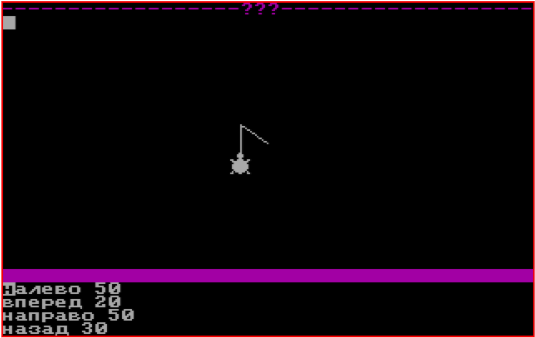
\includegraphics[width=0.6\textwidth]{logo.png}}
			\end{column}
		\end{columns}
		\vspace{0.7cm}
		\center{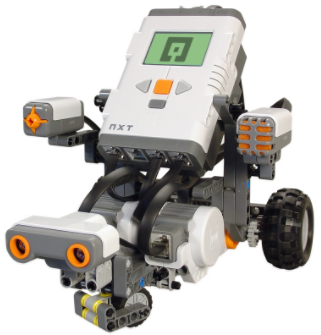
\includegraphics[width=0.2\textwidth]{lego.png}\hspace{2cm}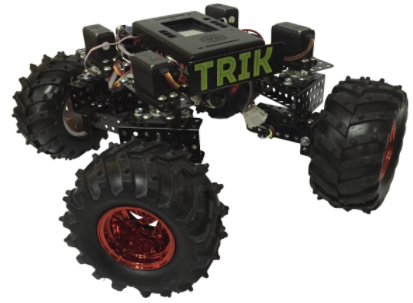
\includegraphics[width=0.3\textwidth]{trik.png}}
	\end{frame}

	\begin{frame}
		\frametitle{Existing visual programming tools for robots}
		\begin{columns}
			\begin{column}{0.6\textwidth}
				\begin{itemize}
					\item NXT-G, EV3-G
					\item Robolab
					\item Scratch
					\begin{itemize}
						\item S4A, mBlock, Enchanting, ScratchDuino, Blockly, App Inventor
					\end{itemize}
					\item 12Blocks
					\item Open Roberta
					\item Ardublock
					\item ...
				\end{itemize}
			\end{column}
			\begin{column}{0.4\textwidth}
				\center{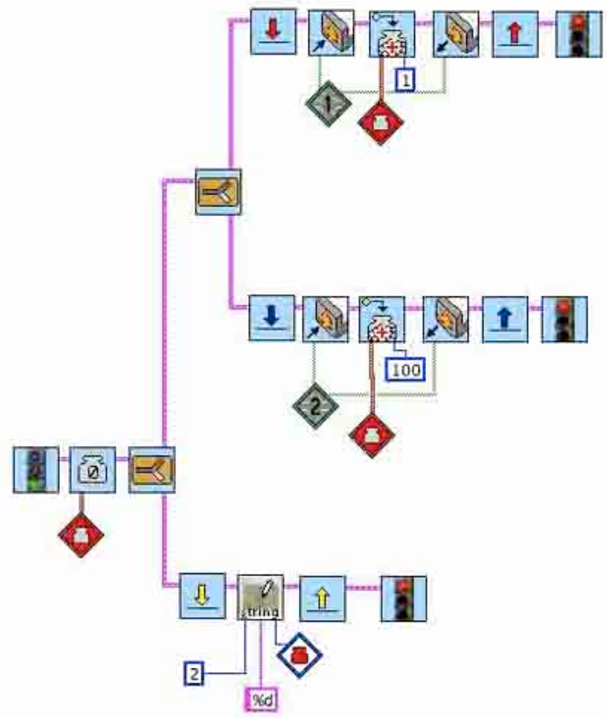
\includegraphics[width=0.8\textwidth]{robolab.png}}
			\end{column}
		\end{columns}
	\end{frame}

	\begin{frame}
		\frametitle{TRIK Studio}
		\begin{itemize}
			\item Lego Mindstorms NXT/EV3 and TRIK robotic kits
			\begin{itemize}
				\item control-flow and data-flow languages
				\item a number of textual languages
			\end{itemize}
			\item Several program execution modes
			\begin{itemize}
				\item 2D simulator
				\item debugging on a PC + sending commands to robots over USB, Bluetooth and Wi-Fi
				\item code generation and binary execution on robots
			\end{itemize}
			\item Cross-platform (Windows, Mac OS X, Linux)
			\item Open-source and free to use
			\begin{itemize}
				\item Third-party plugins, like Pioneer quadcopter or YoTik kit
			\end{itemize}
			\item Currently supports English, Russian and French languages
		\end{itemize}
	\end{frame}

	\begin{frame}
		\frametitle{Visual Language}
		\center{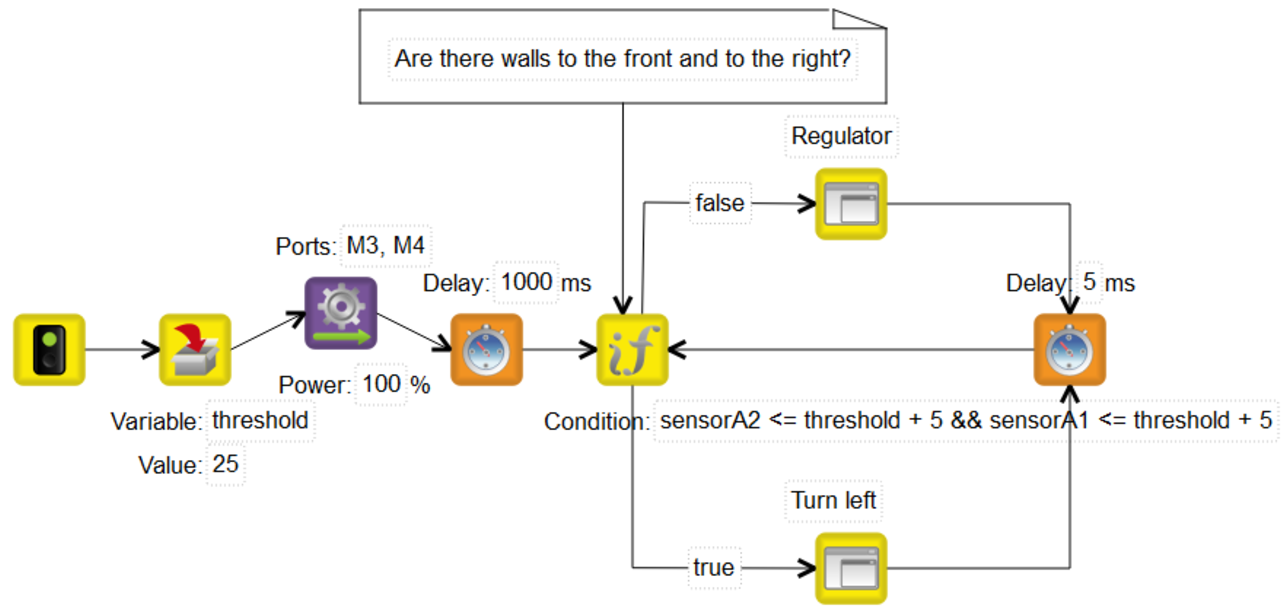
\includegraphics[width=0.9\textwidth]{visualLanguage.png}}
	\end{frame}

	\begin{frame}
		\frametitle{QReal DSM platform}
		\begin{itemize}
			\item Metamodeling tools
			\begin{itemize}
				\item metaeditor, shapes editor etc.
			\end{itemize}
			\item Generic kernel
			\begin{itemize}
				\item common visual IDE tools
			\end{itemize}
			\item Language plugins
			\begin{itemize}
				\item automatically generated from language metamodels
			\end{itemize}
			\item Tool plugins
			\begin{itemize}
				\item code generators, interpreters, version control support, ...
			\end{itemize}
		\end{itemize}
		\begin{textblock}{2}(8,-4)
			
\includegraphics[width=\textwidth]{qrealLogo.png}
		\end{textblock}
	\end{frame}

	\begin{frame}
		\frametitle{Online education}
		\begin{itemize}
			\item MOOC on educational robotics (in Russian)
			\begin{itemize}
				\item \href{https://stepik.org/s/7qe3xj4Z}{https://stepik.org/s/7qe3xj4Z}
			\end{itemize}
			\item Automatic checking of solution correctness
			\begin{itemize}
				\item based on 2D model simulation with specified constraints on robot behavior
			\end{itemize}
			\item Web-based 2D model environment with the ability to replay robot track
		\end{itemize}
	\end{frame}

	\begin{frame}
		\frametitle{Conclusion}
		\begin{itemize}
			\item approx. 10K users across the globe
			\item Russian, English and French languages support
			\item Written in C++/Qt, approx. 100K LOC (+ 120K LOC of QReal core)
			\item Cross-platform, open-source and free to use
			\begin{itemize}
				\item \href{https://github.com/qreal/qreal}{https://github.com/qreal/qreal}
				\item \href{http://blog.trikset.com/p/eng.html}{http://blog.trikset.com/p/eng.html}
			\end{itemize}
		\end{itemize}
	\end{frame}

	\begin{frame}
		\frametitle{Demo}
		\center{\Huge{\textcolor{cadmiumgreen}{Demonstration}}}
	\end{frame}

\end{document}

